\documentclass[t,aspectratio=169,14pt]{beamer}  % [t], [c], или [b] --- вертикальное выравнивание на слайдах (верх, центр, низ)
% \documentclass[handout]{beamer} % Раздаточный материал (на слайдах всё сразу)
% \documentclass[t,aspectratio=169]{beamer} % Соотношение сторон

\usetheme{Madrid}
\usecolortheme{seahorse}

%%% Работа с русским языком
\usepackage{cmap}					% поиск в PDF
%\usepackage{mathtext} 				% русские буквы в формулах
\usepackage[T2A]{fontenc}			% кодировка
\usepackage[utf8]{inputenc}			% кодировка исходного текста
\usepackage[russian]{babel}	% локализация и переносы
\usefonttheme{serif} % default, serif, professionalfonts, structurebold, structureitalicserif,structuresmallcapsserif 
\setbeamerfont{frametitle}{size=\large}
\setbeamerfont{framesubtitle}{size=\normalsize}

%%% Работа с картинками
\usepackage{graphicx}  % Для вставки рисунков
\graphicspath{{images}}  % папки с картинками
\setlength\fboxsep{3pt} % Отступ рамки \fbox{} от рисунка
\setlength\fboxrule{1pt} % Толщина линий рамки \fbox{}
%\usepackage{wrapfig} % Обтекание рисунков текстом
\setbeamertemplate{caption}{\raggedright\insertcaption\par}
%[numbered] % set captions with numbers
%%% Другие пакеты
\usepackage{lastpage} % Узнать, сколько всего страниц в документе.
\usepackage{soul} % Модификаторы начертания
\usepackage{csquotes} % Еще инструменты для ссылок
%\usepackage[style=authoryear,maxcitenames=2,backend=biber,sorting=nty]{biblatex}
\usepackage{multicol} % Несколько колонок
\usepackage{hyperref}
\hypersetup{				% Гиперссылки
	unicode=true,           % русские буквы в раздела PDF
	pdftitle={Запоминать Писание Наизусть},   % Заголовок
	pdfauthor={Библейская церковь Санкт-Петербурга},      % Автор
	pdfsubject={Тема},      % Тема
	pdfcreator={Создатель}, % Создатель
	pdfproducer={Производитель}, % Производитель
	pdfkeywords={keyword1} {key2} {key3}, % Ключевые слова
	colorlinks=false,       	% false: ссылки в рамках; true: цветные ссылки
	linkcolor=red,          % внутренние ссылки
	citecolor=black,        % на библиографию
	filecolor=magenta,      % на файлы
	urlcolor=cyan           % на URL
}

\def\hy#1{\parbox{\linewidth}{#1}} % hypenate text

%-------------------------------------------------------
\title{\textsc{\textbf{Делиться Евангелием}}}
\subtitle{Зачем и Как}
\author[Библейская Церковь СПб]{}

\titlegraphic{\vspace{-1.5cm}
\includegraphics[width=7cm]{bible-church-spb-logo}}
\date{}

% Change example block width
\addtobeamertemplate{block example begin}{%
    \setlength{\textwidth}{0.45\textwidth}
}{}

\usepackage{etoolbox}

\makeatletter
\patchcmd{\beamer@sectionintoc}{\vskip1.5em}{\vskip0.3em}{}{}
\patchcmd{\beamer@subsectionintoc}{\vskip1.5em}{\vskip0.5em}{}{}
\makeatother

\addtobeamertemplate{block begin}{\vfill}{}
\addtobeamertemplate{block end}{}{\vfill}

\AtBeginSection[]
{
  \begin{frame}
    \frametitle{Содержание}
    \tableofcontents[currentsection]
  \end{frame}
}

\begin{document}

\frame[plain]{\titlepage}	% Титульный слайд
%-------------------------------------------------------
\begin{frame}{Содержание}
    \tableofcontents[hideallsubsections]
\end{frame}
%-------------------------------------------------------
\section{Колесо~--- иллюстрация жизни христианина}
\begin{frame}[c]
\frametitle{\insertsection}
	\begin{multicols*}{2}
	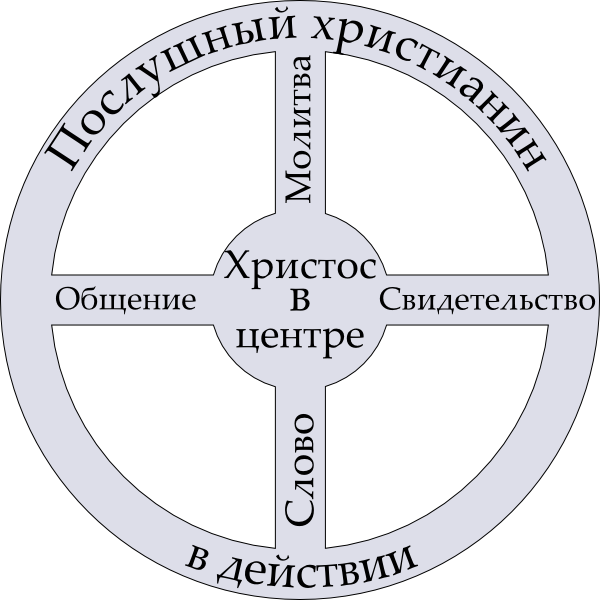
\includegraphics[height=0.8\textheight]{wheel.png}
	\columnbreak
	\pause
	\only<2>{
		\textbf{Христос в центре}
		\begin{itemize}
			\item 2 Коринфянам 5:17
			\item Галатам 2:19б--20
		\end{itemize}

	}
	\only<3>{
		\textbf{Слово}
		\begin{itemize}
			\item Навина 1:8
			\item 2 Тимофею 3:16--17
		\end{itemize}		
	}
	\only<4>{
		\textbf{Молитва}
		\begin{itemize}
			\item Иоанна 15:7
			\item Филлипийцам 4:6--7
		\end{itemize}		
	}
	\only<5>{
		\textbf{Общение}
		\begin{itemize}
			\item Евреям 10:24--25
			\item Матфея 18:20
		\end{itemize}		
	}
	\only<6>{
		\textbf{Свидетельство}
		\begin{itemize}
			\item Матфея 4:19
			\item Римлянам 1:16
		\end{itemize}		
	}
	\only<7>{
		\textbf{Послушный христианин в~действии}
		\begin{itemize}
			\item Римлянам 12:1
			\item Иоанна 14:21
		\end{itemize}		
	}
	\only<8>{
		\textbf{Применение}
		\begin{itemize}
			\item Является ли Христос моей ступицей~--- центром моей жизни?
			\item Все ли спицы в~моём колесе?
			\item Какие спицы короче и~нуждаются в~росте?
			\item Послушен ли я Христу?
		\end{itemize}		
	}	
\end{multicols*}
\end{frame}
%-------------------------------------------------------
\section{Свидетельство. Заповеди}
%-------------------------------------------------------
\begin{frame}
	\frametitle{\insertsection}

	\begin{block}{Матфея 4:18-20}
		Проходя же близ моря Галилейского, Он увидел двух братьев, Симона, называемого Петром, и Андрея, брата его, закидывающих сети в море; 
		ибо они были рыболовы; и говорит им: \vspace{0.3cm}
		\linebreak идите за Мною, и Я сделаю вас ловцами человеков. \vspace{0.3cm}
		\linebreak И они тотчас, оставив сети, последовали за Ним.
	\end{block}
\end{frame} 
%-------------------------------------------------------
\begin{frame}
	\frametitle{\insertsection}

	\begin{block}{Матфея 24:14}
		И проповедано будет сие Евангелие Царствия\linebreak по всей вселенной,\linebreak 
		во свидетельство всем народам;\linebreak
		и тогда придет конец.
	\end{block}

\end{frame}
%-------------------------------------------------------
\begin{frame}
	\frametitle{\insertsection}

	\begin{block}{Матфея 28:18-20, Современный перевод}
		Иисус подошел и заговорил с ними. Он сказал:\vspace{0.3cm}
		
		«Мне дана вся власть на небе и на земле.\linebreak 
		Итак, \linebreak  \hphantom{aaa}ступайте \linebreak и \hphantom{a}сделайте все народы Моими учениками. \linebreak 
		\hphantom{aaa}Крестите их во имя Отца, Сына и Святого Духа \linebreak 
		и \hphantom{a}научите соблюдать всё, что Я вам повелел. \linebreak 
		И \hphantom{a}знайте: Я с вами всегда, до конца мира».
	\end{block}
\end{frame}
%-------------------------------------------------------
\begin{frame}
	\frametitle{\insertsection}

	\begin{block}{Деяния 1:8}
		но вы \linebreak 
		\hphantom{a} примете силу, \hphantom{M}когда сойдёт на вас Дух Святый;\linebreak 
		и будете Мне свидетелями \linebreak 
		\hphantom{MM} в~Иерусалиме \linebreak
		\hphantom{MM} и во всей Иудее \linebreak
		\hphantom{MM} и Самарии \linebreak
		\hphantom{MM} и даже до края земли.
	\end{block}
\end{frame} 
%-------------------------------------------------------
\section{Пример Иисуса}

\begin{frame}
	\frametitle{\insertsection}

\begin{itemize}
	\item Нужды
	\item Новые сообщества
\end{itemize}

\end{frame}
%-------------------------------------------------------
\section{В\'{и}дение}
\begin{frame}[c]
	\frametitle{\insertsection}
	\framesubtitle{\insertsubsection}

\end{frame}
%-------------------------------------------------------
\section{Поднимите флаг}
\begin{frame}[c]
	\frametitle{\insertsection}
	% \framesubtitle{\insertsubsection}
	\begin{block}{}
		Поднять флаг~--- показать окружающим вашу веру.
	\end{block}	
	Идеи:
	\begin{itemize}
		\item Библия на виду
		\item Расскажите историю своего пути к~вере
		\item Расскажите историю веры из вашей жизни
		\item Предложите помолиться
		\item Используйте мессенджеры и~социальные сети
	\end{itemize}
\end{frame}
%-------------------------------------------------------
\begin{frame}[c]
	\frametitle{Мессенджеры и~социальные сети}
	\framesubtitle{Поднимите флаг}
	\begin{figure}[h]
		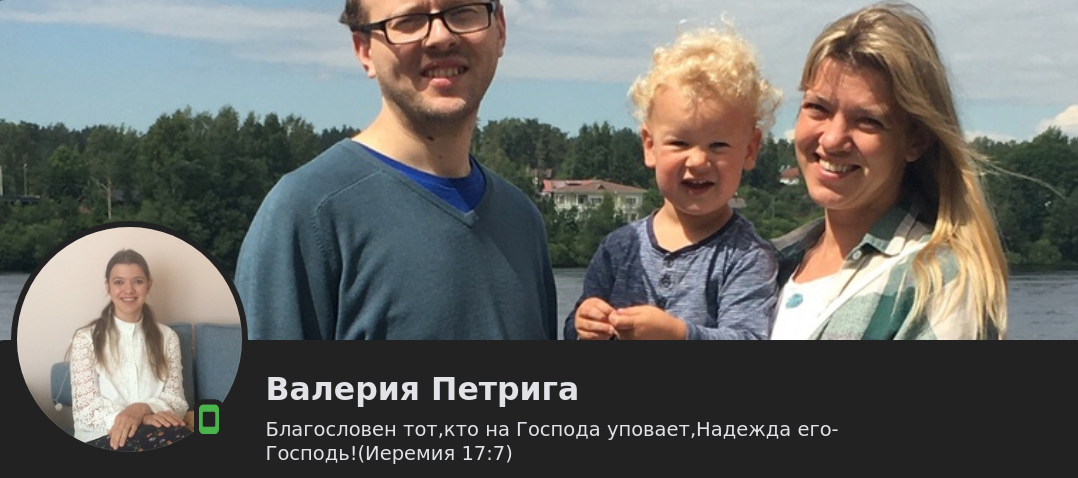
\includegraphics[height=0.63\textheight]{vk.png}
		\caption{ВКонтакте. Страница}
		\end{figure}
\end{frame}
%-------------------------------------------------------
\begin{frame}[c]
	\frametitle{Мессенджеры и~социальные сети}
	\framesubtitle{Поднимите флаг}
	\begin{multicols*}{2}

		\only<1>{
		\begin{figure}[h]
		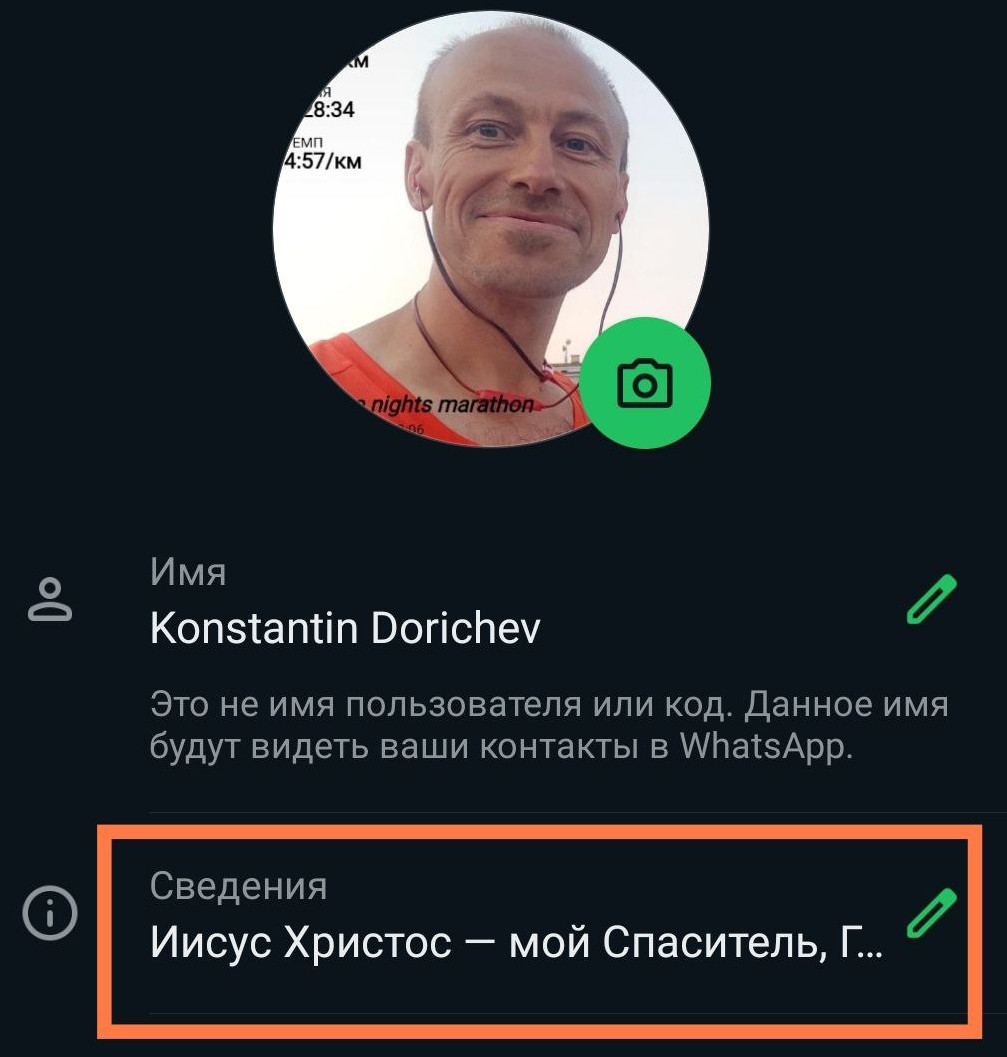
\includegraphics[height=0.63\textheight]{whatsapp_profile.jpg}
		\caption{WhatsApp. Профиль}
		\end{figure}
		\columnbreak
		\begin{figure}[h]
			\includegraphics[height=0.63\textheight]{whatsapp.jpg}
			\caption{WhatsApp. Статус}
		\end{figure}		
		}

		\only<3>{
		\begin{figure}[h]
		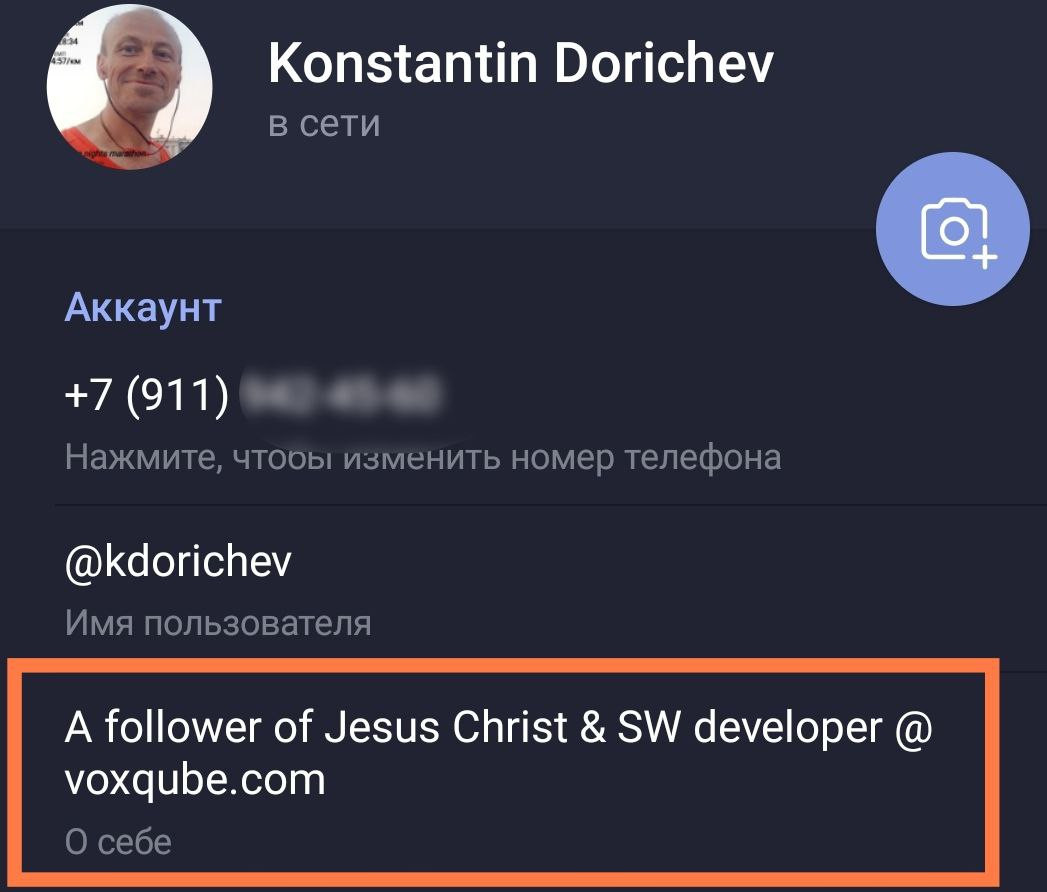
\includegraphics[height=0.63\textheight]{telegram.jpg}
		\caption{Телеграм. Профиль}
		\end{figure}
		\columnbreak

		\begin{figure}[h]
			 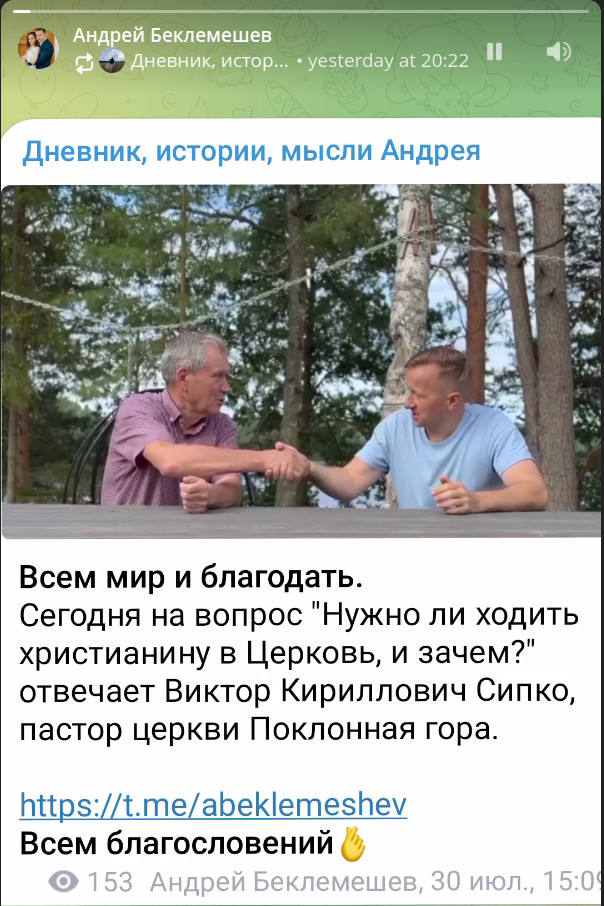
\includegraphics[height=0.63\textheight]{telegram-story.jpg}
			\centering
			\caption{Телеграм. Истории}
		\end{figure}		
		}

		\only<2>{
			\begin{figure}[h]
				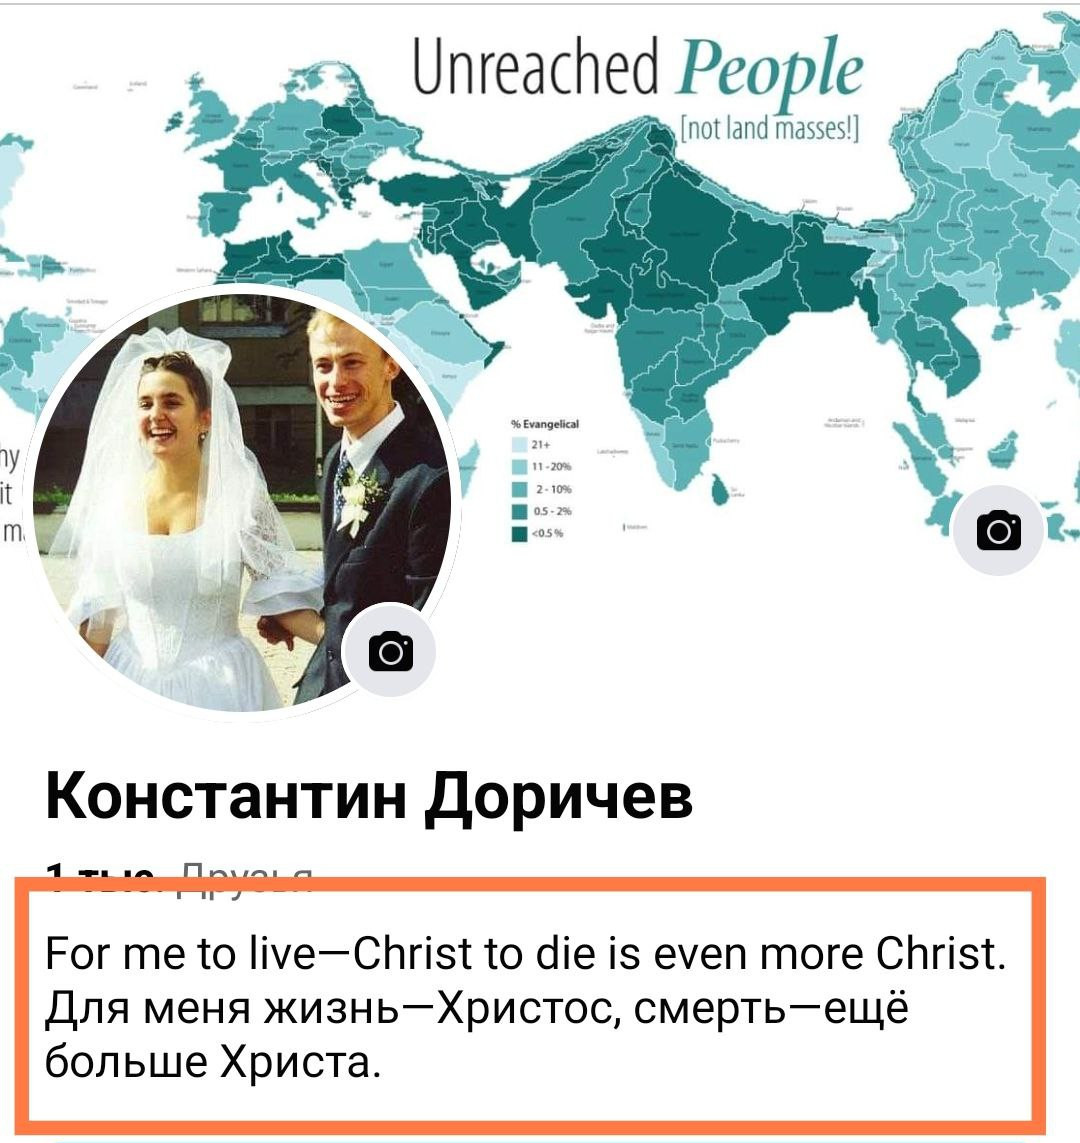
\includegraphics[height=0.63\textheight]{facebook.jpg}
				\caption{Facebook. Профиль}
				\end{figure}
				\columnbreak
		
				\begin{figure}[h]
					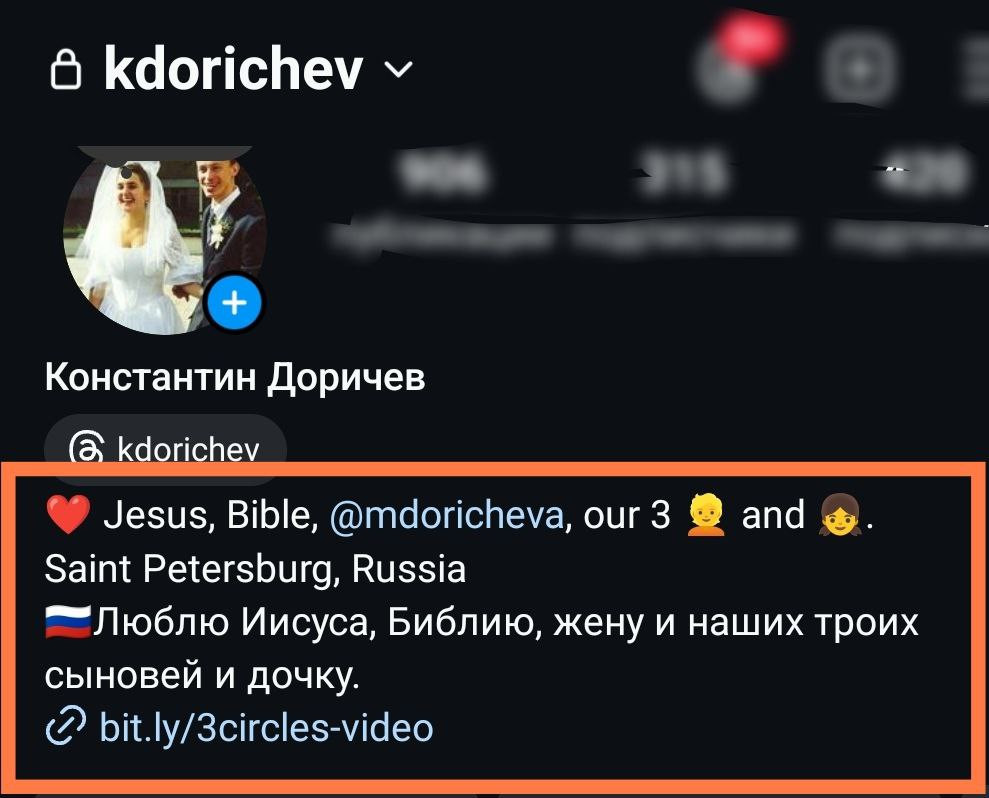
\includegraphics[height=0.63\textheight]{instagram.jpg}
					\caption{Instagram. Профиль}
					\end{figure}	
		}
	
	\end{multicols*}
\end{frame}	
%-------------------------------------------------------
\section{Отклики на Евангелие}
\begin{frame}[c]
	\frametitle{\insertsection}
	\framesubtitle{Проповедь Павла в Афинах}
	\begin{block}{Деяния 17:32-34}
		Услышав о~воскресении мертвых,\linebreak
		\hphantom{M}одни насмехались,\linebreak
		\hphantom{M}а~другие говорили: об этом послушаем тебя в другое время\ldots \linebreak
		\hphantom{M}Некоторые же мужи, пристав к нему, уверовали\ldots
	\end{block}	
\end{frame}	
%-------------------------------------------------------
\begin{frame}[c]
	\frametitle{\insertsection}
	\framesubtitle{Светофор}

	\begin{multicols*}{2}

		\begin{figure}[h]
		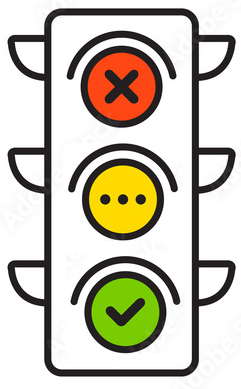
\includegraphics[height=0.4\textheight]{svetofor.png}
		\end{figure}
		\columnbreak

		Отклик на Евангелие:
		\begin{itemize}
			\item Красный~--- Нет!
			\item Жёлтый~--- Интересно
			\item Зелёный~--- Да!
			\item Уже верующий
		\end{itemize}	
	\end{multicols*}
\end{frame}
%-------------------------------------------------------
\section{Три Круга}
\begin{frame}[c]
	\frametitle{\insertsection}
	\framesubtitle{Презентация Евангелия}
	\begin{figure}[h]
		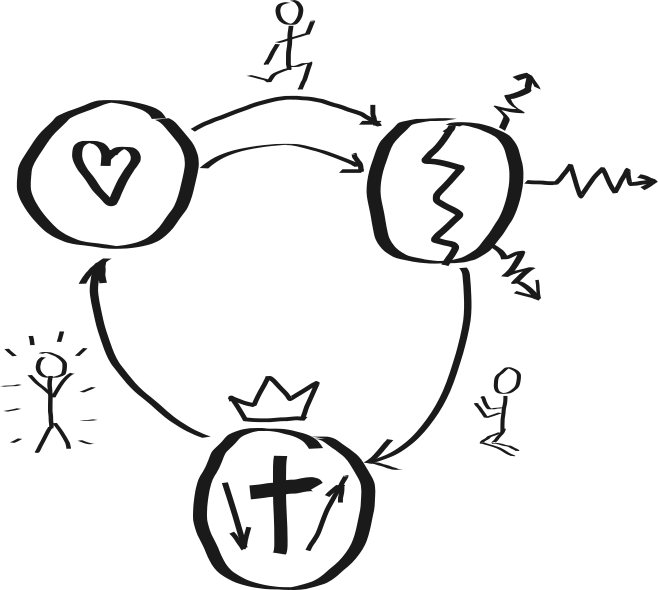
\includegraphics[height=0.76\textheight]{3circles.png}
	\end{figure}
\end{frame}
%-------------------------------------------------------
\section{Практика}
\begin{frame}[c]
\frametitle{\insertsection}
\begin{block}{}
	\centering \Huge Потренируемся!
\end{block}
\end{frame}
\end{document}
